\documentclass[12pt,parskip]{komatufte}
\usepackage[subpreambles=false]{standalone}

%%%%%%%%%%%%%%%%%%%%%%%%%%%
% Silence warning messages
\usepackage{silence}
\WarningsOff[scrlayer-notecolumn]
\WarningsOff[biblatex]

%%%%%%%%%%%%%%%%%%%%
% Commenting

%\usepackage[author=Lyndon]{pdfcomment}
%\newcommand{\pdfcomment}[1]{} %ignore all comments

%\usepackage{todonotes}
%\newcommand{\pdfcomment}{\todo}


%%%%%%%%%%%%%%%%%%%%
% Tables
\usepackage{booktabs}

%%%%%%%%%%%%%%%%%%%
% Fonts
\usepackage{tgadventor} %sans
\usepackage{tgpagella}  %serif
\usepackage{inconsolata} %mono
\usepackage[T1]{fontenc}

\usepackage{microtype}
\usepackage[all]{nowidow}
%%%%%%%%%%%%%%%%%%%%%%%
% Styling
\setcounter{secnumdepth}{4}
\setcounter{tocdepth}{2}

\usepackage{placeins}



%%%%%%%%%%%%%%%%%%%
% Math
\usepackage{amsmath, amssymb, stmaryrd, mathtools}
\DeclareMathOperator*{\argmin}{argmin}
\DeclareMathOperator*{\argmax}{argmax}

\usepackage{xparse,xstring,etoolbox}
% crossref this against notation section
\newcommand{\vv}[1]{\tilde{#1}} % vector
\newcommand{\seq}[1]{\mathcal{#1}} % sequence
\newcommand{\set}[1]{\mathbb{#1}} % set

%%%%%%%%%
% Indexing/sequence indexing
\newcommand{\seqind}[2]{#1^{#2}} % seqence index
\newcommand{\ind}[2]{#1_{#2}} % indexed
\newcommand{\disamb}[2]{#1^{\mathrm{#2}}} %disambiguated

%% Smart indexing and naming
\newcommand{\ifupper}[3]{
    \normalexpandarg
	\exploregroups
	\StrCount{ABCDEFGHIJKLMNOPQRSTUVWXYZ}{#1}[\uppercount]
	\ifnumgreater{\uppercount}{0}{#2}{#3}
}

%smart index
\DeclareDocumentCommand{\ii}{u{_} m}{
	\ifupper{#1}%
	{% just a single uppercase character, i.e. a matrix
		  %make sure the index is the right length
		\StrCount{#2}{,}[\indcount]
		\ifnumgreater{\indcount}{0}
		{ % Got multiple indexes so all good
		 	\ind{#1}{#2}
		}
		{ % Only 1 index so grab the column
		 	\ind{#1}{{:,#2}}
		}
	}%
	{% Not just a single upper case character
		\ind{#1}{#2}
	}
}

\DeclareDocumentCommand{\nn}{u{_} m}{
	\seqind{#1}{#2}
}

\DeclareDocumentCommand{\dd}{u{_} m}{
	\disamb{#1}{#2}
}

% Index of a vector
\DeclareDocumentCommand{\iv}{u{_} m}{\ii{\vv #1}_{#2}}
\DeclareDocumentCommand{\dv}{u{_} m}{\dd{\vv #1}_{#2}}
\DeclareDocumentCommand{\nv}{u{_} m}{\nn{\vv #1}_{#2}}

%exp
\let\oldexp\exp
\renewcommand{\exp}[1]{\oldexp \left( #1 \right)}
\newcommand{\exptwo}[1]{\oldexp_2 \left( #1 \right)}

\newcommand{\softmax}{\mathrm{smax}}

\DeclareMathOperator*{\expectedop}{\mathbb{E}}
\DeclareDocumentCommand{\expected}{u{_} m}{
	\expectedop\limits_{\mathrlap{#2}}
}

%%%%%%%%%%%%%%%%
%Graphics
\usepackage{tikz}
\usetikzlibrary{positioning, fit,  shapes.geometric}
\usepackage{ifthen}
\usepackage{etoolbox}

\tikzset{
	backgroundcolor/.style ={fill=white},
	every node/.append style={
		minimum height=7mm,
	},
	labe/.append style={
		%Blue,
		align = center,
		backgroundcolor,
		fill opacity=0.6,
		text opacity=1,
		font={\footnotesize\itshape}	
	},
	layer/.append style={
		draw,
		align = center,
		minimum height=7mm,
	},
	tight/.append style={
		inner sep=0.2mm,
	},
	lookupbox/.append style={
		draw=none,
		append after command={
		       	[shorten <= -0.5\pgflinewidth]
		       	([shift={(-1.5\pgflinewidth,-0.5\pgflinewidth)}]\tikzlastnode.north east)
		       	edge([shift={( 0.5\pgflinewidth,-0.5\pgflinewidth)}]\tikzlastnode.north west) 
		       	([shift={( 0.5\pgflinewidth,-0.5\pgflinewidth)}]\tikzlastnode.north west)
		       	edge([shift={( 0.5\pgflinewidth,-1.5\pgflinewidth)}]\tikzlastnode.south west)            
		       	([shift={( -1.5\pgflinewidth,+0.5\pgflinewidth)}]\tikzlastnode.south east)
		       	edge([shift={(-1.5\pgflinewidth,-0.5\pgflinewidth)}]\tikzlastnode.north east)
		},
		inner sep=0.7mm,
		outer sep=0mm,
		minimum width=25mm
	}
}

\usepackage{pgfplots}
\pgfplotsset{compat=1.14}
\pgfplotsset{sideplot/.append style={
		width=\notescolwidth,
		domain=-10:10,
		samples=101,
		smooth,
		enlarge y limits={abs=2},
		axis lines=middle,
		xlabel  = $z$,
		ylabel  = $y$,
	},
	equ/.append style={
		color=blue,
		thick,
		mark=none
	}
}

% Function  For a plot 
% it  needs to be declared in preamble because of how \makenote* interacts with multiple files
\def\errorsurface(#1,#2){(0.5*#1 + 0.7*#2 + sin(deg(1.5*#1 + #2^2)))^2}


\usepackage{graphicx}
\graphicspath{{./figs/}, {./}, {./figs/chaptersentencerrepr/}, {./figs/chapterintromachinelearning/}, {./figs/chapterwordrepr/}}
\usepackage{adjustbox}


%%%%%%%%%%%%%%%%%%%
% Refs
\usepackage{cleveref}

\addbibresource{master.bib}

%%%%%%%%%%%%%%%%%%%%
% Formatting

% for examples from natural language space.
\newcommand{\natlang}[1]{\ifmmode \text{``\texttt{#1}''} \else {``\texttt{#1}''}\fi}
% \ifmmode ``trick'' from https://tex.stackexchange.com/a/15194/5834

%%%%%%%%%%%%%%%%%%%%%



\begin{document}

\setchapterpreamble{%
	\dictum[\textit{English Composition and Literature}, Webster, 1923]
	{
		A sentence is a group of words expressing a complete thought.
	}
}
\chapter{Sentence Representations and Beyond}\label{sec:sentence-representations-and-beyond}
\begin{abstract}
	This chapter discusses representations for larger structures in natural language.
	The primary focus is on the sentence level.
	However, many of the techniques also apply to sub-sentence structures (phrases), and super-sentence structures (documents).
	The three main types of representations discussed here are: unordered models, such as sum of word embeddings; sequential models, such as recurrent neural networks; and structured models, such as recursive autoencoders.
\end{abstract}


\aside[Word Embeddings as a by-product]{
	Many sentence representation methods produce word embeddings as a by-product.
	These word embeddings are either output embeddings, from the softmax,
	or input embeddings from a lookup layer.}
\aside[Initialising input embeddings]{
	It is common (but not ubiquitous) to initialise the input embeddings using pretrained embeddings from one of the methods discussed in \Cref{sec:word-representations},
	then allow them to be fine-tuned while training the sentence representation method.
}


It can be argued that the core of true AI,
is  in capturing and manipulating the representation of an idea.
In natural language a sentence (as defined by Webster in the quote above),
is such a representation of an idea, but it is not machine manipulatable.
As such the conversion of sentences to a machine manipulatable representation is an important task in AI research.


All techniques which can represent documents (or paragraphs) by necessity represent sentences as well.
A document (or a paragraph), can consist only of a single sentence.
Many of these models always work for sub-sentence structures also, like key-phrases.
When considering representing larger documents,
neural network embedding models directly compete with vector information retrieval models,
such as LSI \pcite{dumais1988using}, probabilistic LSI \pcite{hofmann2000learning} and  LDA \pcite{blei2003latent}.


\aside[Word Sense Embeddings in Sentence Embeddings]{
While the \Cref{sec:word-sense-representations} was all about sense embeddings, they are unmentioned here.
One might think that they would be very useful for sentence embeddings.
However, they are not as needful as one might expect.
The sense of a word being used is determined by the context.
Ideally, it is determined by what the context means.
As a sentence embedding is a direct attempt to represent the meaning of such a context, determining the sense of each word within it is not required.
Using sense embeddings instead of word embeddings is a valid extension to many of these methods.
However it requires performing word sense disambiguation,
which as discussed is very difficult.
}



\section{Unordered and Weakly Ordered Representations}

A model that does not take into account word order cannot perfectly capture the meaning of a sentence.
\tcite{Mitchell2008} give the poignant examples of:
\begin{itemize}
	\item \natlang{It  was  not  the  sales  manager who  hit  the  bottle that day, but the office worker with the serious drinking problem.}
	\item \natlang{That  day  the  office  manager,   who  was drinking, hit the problem sales worker with a bottle, but it was not serious.}
\end{itemize}
These two sentences have the same words, but in a different structure, resulting in their very different meanings.
In practice, however, representations which discard word order can be quite effective.


\subsection{Sums of Word Embeddings}
\aside[SOWE is the product of the BOW with an embedding matrix]{
	The reader may recall from \Cref{sec:word-representations},
	that a word-embedding lookup is the same as a one-hot vector product:
	$\i C_{\n w_i} = C\,\hat{e}_{\n w_i}$.
	Similar can be said for sum of word embeddings (SOWE) and bag of words (BOW).
	For some set of words $\seq{W} = \lbrace{w_1,\ldots, w_n \rbrace}$:
	the BOW representation is $B_\seq{W} = \sum_{\n w_i\in \seq{W}} \hat{e}_{\n w_i}$;
	the SOWE representation is $\sum_{\n w_i\in \seq{W}} C_{\n w_i} = CB_\seq{W}$.
	As with word-embeddings, it is immensely cheaper to calculate this via lookup and sum, rather than via matrix product;
	except on systems with suitable sparse matrix product tricks.	
}

Classically, in information retrieval, documents have been represented as bags of words (BOW).
That is to say a vector with length equal to the size of the vocabulary, with each position representing the count of the number of occurrences of a single word.
This is much the same as a \emph{one-hot vector} representing a word, but with every word in the sentence/document counted.
The word embedding equivalent is sums of word embeddings (SOWE), and mean of word embeddings (MOWE).
These methods, like BOW, lose all order information in the representation.
In many cases it is possible to recover a BOW from a much lower dimensional SOWE  \pcite{White2015BOWgen}.

Surprisingly, these unordered methods have been found on many tasks to be extremely well performing, better than several of the more advanced techniques discussed later in this chapter.
This has been noted in several works including: \tcite{White2015SentVecMeaning}, \tcite{RitterPosition} and \tcite{rui2017mvrusemantic}.
It has been suggested that this is because in English there are only a few likely ways to order any given bag of words.
It has been noted that given a simple n-gram language model the original sentences can often be recovered from BOW \pcite{Horvat2014} and thus also from a SOWE \pcite{White2016a}.
Thus word-order may not in-fact be as important as one would expect in many natural language tasks, as it is in practice more proscribed than one would expect.
That is to say very few sentences with the same word content, will in-practice be able to have it rearranged for a very different meaning.
However, this is unsatisfying, and certainly cannot capture fine grained meaning.


The step beyond this is to encode the n-grams into a bag of words like structure.
This is a bag of n-grams (BON), e.g. bag of trigrams.
Each index in the vector thus represents the occurrence of an n-gram in the text.
So \natlang{It is a good day today}, has the trigrams: \natlang{(It is a)},\natlang{(is a good)},\natlang{(a good day)}, \natlang{(good day today)}.
As is obvious for all but the most pathological sentences, recovering the full sentence order from a bag of n-grams is possible even without a language model.

The natural analogy to this with word embeddings might seem to be to find n-gram embeddings by the concatenation of $n$ word embeddings; and then to sum these.
However, such a sum is less informative than it might seem.
As the sum in each concatenated section is equal to the others, minus the edge words.


% To illustrate the case of trigram sums of word embeddings, for \natlang{It is a good day today},
%the sums in each position would be:
%\begin{multline}
%\left[\begin{array}{c|c|c}
%	\sum & \sum & \sum\\
%	\i C_{it} & \i C_{was} & \i C_{a}\\
%	\i C_{was} & \i C_{a} & \i C_{good}\\
%	\i C_{a} & \i C_{good} & \i C_{day}\\
%	\i C_{good} & \i C_{day} & \i C_{today}
%\end{array}\right]\\
%=\left[\begin{array}{c|c|c}
%	\i C_{M}+\i C_{it}-\i C_{day} & \i C_{M} & \i C_{M}-\i C_{was}+\i C_{today}\end{array}\right]
%\end{multline}
%\pdfcomment{remove one or both of these}
%\begin{multline}
%\left[\begin{array}{c|c|c}
%	\quad \i C_{\n w_{1}} & \quad \i C_{\n w_{2}} & \quad \i C_{\n w_{3}}\\
%	+\i C_{\n w_{2}} & +\i C_{\n w_{3}} & +\i C_{\n w_{4}}\\
%	+\i C_{\n w_{3}} & +\i C_{\n w_{4}} & +\i C_{\n w_{5}}\\
%	+\i C_{\n w_{4}} & +\i C_{\n w_{5}} & +\i C_{\n w_{6}}
%\end{array}\right]=\\
%\left[\begin{array}{c|c|c}
%	\sum \i C_{\n w_{i}}-\i C_{\n w_{n-1}}-\i C_{\n w_{n-2}} & \sum \i C_{\n w_{i}}-\i C_{\n w_{1}}-\i C_{\n w_{n-1}} & \sum \i C_{\n w_{i}}-\i C_{\n w_{1}}-\i C_{\n w_{2}}\end{array}\right]
%\end{multline}


Instead one should train an n-gram embedding model directly.
The method discussed in \Cref{sec:word-representations}, can be adapted to use n-grams rather than words as the basic token.
This was explored in detail by \pcite{li2017neural}.
Their model is based on the skip-gram word embedding method.
They take as input an n-gram embedding, and attempt to predict the surrounding n-grams.
This reduces to the original skip-gram method for the case of unigrams.
Note that the surrounding n-grams will overlap in words (for $n>1$)  with the input n-gram.
As the overlap is not complete, this task remains difficult enough to encourage useful information to be represented in the embeddings.
\textcite{li2017neural} also consider training n-gram embeddings as a bi-product of text classification tasks.



\subsection{Paragraph Vector Models (Defunct)}

\aside[Window vs Context]{
It is important to be clear in this section on the difference between the window and the context.
The window is the words near the target word.
The context (in this context) refers to the larger structure (sentence, paragraph, document) that a representation is attempting to be found for.
The window is always a subset of the context.
In modelling the context many windows within it will be considered (one per target word).
Some works say sentence vector, document vector or paragraph vector.
We say context vector as it could be any of the above.
In theory it could even be a whole collection of documents.
}



\tcite{le2014distributed} introduced two models for representing documents of any length by using augmented word-embedding models.
The models are called Paragraph Vector Distributed Memory (PV-DM) model,
and the Paragraph Vector Distributed Bag of Words  model (PV-DBOW).
The name Paragraph Vector is a misnomer, it function on texts of any length and has most often (to our knowledge) been applied to documents and sentences rather than any in-between structures.
The CBOW and skip-gram models are are extended with an additional context vector that represents the current document (or other super-word structure, such as sentence or paragraph).
This, like the word embeddings, is initialised randomly, then trained during the task.
\textcite{le2014distributed} considered that the context vector itself must contain useful information about the context.
The effect in both cases of adding a context vector is to allow the network to learn a mildly different accusal language model depending on the context.
To do this, the context vector would have to learn a representation for the context.


\aside[PV Model Implementations]{
There is a popular third-party implementation of both the paragraph vector models, under the name \texttt{doc2vec} in the python gensim library \parencite{rehurek_lrec}, along with many information retrieval vector models such as LDA.
}

PV-DBOW is an extension of CBOW.
The inputs to the model are not only the word-embedding $\i C_{w_j}$ for the words $\n w_j$ from the window,
but also a context-embedding $\i D_{\n d_k}$ for its current context (sentence, paragraph or document ) $\n d_k$.
The task remains to predict which word was the missing word from the center of the context $\n w_i$.
\begin{align}
P(\n w_i & \mid \n d_k,\, \n w_{i-\frac{n}{2}},..., \n w_{i-1}, \n w_{i+1},...,\n w_{i+\frac{n}{2}})  \nonumber
\\  & = \softmax(W\i D_{\n d_k} + U \sum_{j=i+1}^{j=\frac{n}{2}} \left( \i C_{\n w_{i-j}}+\i C_{\n w_{i+j}} \right))
\end{align}


PV-DM is the equivalent extension for skip-grams.
Here the input to the model is not only the central word, but also the context vector.
Again, the task remains to predict the other words from the window.
\begin{equation}
P(\n w_j \mid \n d_k,\, \n w_{i}) = \left[ \softmax(W\i D_{\n d_k} + V\,\i C_{\n w_{i}}) \right]_{w_j} 
\end{equation}


The results of this work are now considered of limited validity.
There were failures to reproduce the reported results in the original evaluations
which were on sentiment analysis tasks.
These were documented online by several users, including by the second author.%
\footnote{ \url{https://groups.google.com/forum/\#!msg/word2vec-toolkit/Q49FIrNOQRo/DoRuBoVNFb0J}}
A follow up paper, \tcite{mesnil2014ensemble} found that reweighed bags of n-grams \pcite{wang2012baselines} out performed the paragraph vector models.
Conversely, \textcite{lau2016doc2vecissues} found that on short text-similarity problems, with the right tuning, the paragraph vector models could perform well;
however they did not consider the reweighed n-grams of \parencite{wang2012baselines}.
On a different short text task, \textcite{White2015SentVecMeaning} found the paragraph vector models to significantly be out-performed by SOWE, MOWE, BOW, and BOW with dimensionality reduction.
This highlights the importance of rigorous testing against a suitable baseline, on the task in question.




\section{Sequential Models}

\begin{figure}
	\caption{The unrolled structure of an RNN for use in (a) Matched-sequence (b) Encoding, (c) Decoding and (d) Encoding-Decoding (sequence-to-sequence) problems. RU is the recurrent unit -- the neural network which reoccurs at each time step. (Repeated from \Cref{fig-rnns})
	}
	\label{fig-rnns-sq}
	
	\resizebox{\textwidth}{!}{\documentclass[landscape]{article}
\usepackage[a3paper]{geometry}

\usepackage{tikz}
\usetikzlibrary{positioning, fit,  shapes.geometric}
\usepackage{ifthen}
\usepackage{etoolbox}

\tikzset{
	backgroundcolor/.style ={fill=white},
	every node/.append style={
		minimum height=7mm,
	},
	labe/.append style={
		%Blue,
		align = center,
		backgroundcolor,
		fill opacity=0.6,
		text opacity=1,
		font={\footnotesize\itshape}	
	},
	layer/.append style={
		draw,
		align = center,
		minimum height=7mm,
	},
	tight/.append style={
		inner sep=0.2mm,
	},
	lookupbox/.append style={
		draw=none,
		append after command={
		       	[shorten <= -0.5\pgflinewidth]
		       	([shift={(-1.5\pgflinewidth,-0.5\pgflinewidth)}]\tikzlastnode.north east)
		       	edge([shift={( 0.5\pgflinewidth,-0.5\pgflinewidth)}]\tikzlastnode.north west) 
		       	([shift={( 0.5\pgflinewidth,-0.5\pgflinewidth)}]\tikzlastnode.north west)
		       	edge([shift={( 0.5\pgflinewidth,-1.5\pgflinewidth)}]\tikzlastnode.south west)            
		       	([shift={( -1.5\pgflinewidth,+0.5\pgflinewidth)}]\tikzlastnode.south east)
		       	edge([shift={(-1.5\pgflinewidth,-0.5\pgflinewidth)}]\tikzlastnode.north east)
		},
		inner sep=0.7mm,
		outer sep=0mm,
		minimum width=25mm
	}
}
\usepackage{amsmath, amssymb, stmaryrd, mathtools}
\DeclareMathOperator*{\argmin}{argmin}
\DeclareMathOperator*{\argmax}{argmax}

\usepackage{xparse,xstring,etoolbox}
% crossref this against notation section
\newcommand{\vv}[1]{\tilde{#1}} % vector
\newcommand{\seq}[1]{\mathcal{#1}} % sequence
\newcommand{\set}[1]{\mathbb{#1}} % set

%%%%%%%%%
% Indexing/sequence indexing
\newcommand{\seqind}[2]{#1^{#2}} % seqence index
\newcommand{\ind}[2]{#1_{#2}} % indexed
\newcommand{\disamb}[2]{#1^{\mathrm{#2}}} %disambiguated

%% Smart indexing and naming
\newcommand{\ifupper}[3]{
    \normalexpandarg
	\exploregroups
	\StrCount{ABCDEFGHIJKLMNOPQRSTUVWXYZ}{#1}[\uppercount]
	\ifnumgreater{\uppercount}{0}{#2}{#3}
}

%smart index
\DeclareDocumentCommand{\ii}{u{_} m}{
	\ifupper{#1}%
	{% just a single uppercase character, i.e. a matrix
		  %make sure the index is the right length
		\StrCount{#2}{,}[\indcount]
		\ifnumgreater{\indcount}{0}
		{ % Got multiple indexes so all good
		 	\ind{#1}{#2}
		}
		{ % Only 1 index so grab the column
		 	\ind{#1}{{:,#2}}
		}
	}%
	{% Not just a single upper case character
		\ind{#1}{#2}
	}
}

\DeclareDocumentCommand{\nn}{u{_} m}{
	\seqind{#1}{#2}
}

\DeclareDocumentCommand{\dd}{u{_} m}{
	\disamb{#1}{#2}
}

% Index of a vector
\DeclareDocumentCommand{\iv}{u{_} m}{\ii{\vv #1}_{#2}}
\DeclareDocumentCommand{\dv}{u{_} m}{\dd{\vv #1}_{#2}}
\DeclareDocumentCommand{\nv}{u{_} m}{\nn{\vv #1}_{#2}}

%exp
\let\oldexp\exp
\renewcommand{\exp}[1]{\oldexp \left( #1 \right)}
\newcommand{\exptwo}[1]{\oldexp_2 \left( #1 \right)}

\newcommand{\softmax}{\mathrm{smax}}

\DeclareMathOperator*{\expectedop}{\mathbb{E}}
\DeclareDocumentCommand{\expected}{u{_} m}{
	\expectedop\limits_{\mathrlap{#2}}
}

\begin{document}

\numdef{\N}{8}
\numdef{\labelwidth}{5.5cm}
%%%%%%%%%%%%%%%%%%%%%%%%%
% Encoder

\begin{tikzpicture}[]

\begin{scope}
	\node(lblEncoder)[text width= \labelwidth] {\textbf{RNN Encoder:}\\%
	Variable $n$ inputs: $\nv x_t$\\%
	1 output: $\hat{y}$ \\%
	};
	
	\coordinate (L0) at (lblEncoder.east);
	
	\foreach \I[count=\j from 0] in {1,...,\N}{
		\ifnumequal{\I}{\N - 1}{%
			\node(L\I)[dashed, layer, right = of L\j] {...};
			\node(w\I)[below = of L\I]{...};
		}%
		{	
			\node(L\I)[layer, right = of L\j] {RU};
			\node(w\I)[below = of L\I]{\ifnumequal{\I}{\N}{$\nv x_n$}{$\nv x_\I$}};
			\draw[->](w\I) -- (L\I);
		}
	}
	\foreach \I[count=\j from 1] in {2,...,\N} {
		\draw[->] (L\j) edge node[labe]{state} (L\I);
	}
	
	\node(out) [above = of L\N]{$\hat{y}$};
	\draw[->] (L\N) -- (out);
\end{scope}

%%%%%%%%%%%%%%%%
% Decoder
\begin{scope}[yshift=-5cm] 
\node(lbl)[text width= \labelwidth] {\textbf{RNN Decoder:}\\%
1 input: $x$\\%
variable $m$ outputs: $\n \hat{y}_t$ \\%
with prompts: $\nv r_t$ (often $\nv y_{t-1}$)
};

\coordinate (L0) at (lbl.east);
\coordinate (L1c)[right = of L0];
\node(x)[below right = 4 of L1c]{$x$};

\foreach \I[count=\j from 0] in {1,...,\N}{
	\ifnumequal{\I}{\N - 1}{%
		\node(L\I)[dashed, layer, right = of L\j] {...};
		\node(w\I)[above = of L\I]{...};
		\node(y\I)[below = of L\I]{...};
	}%
	{	
		\node(L\I)[layer, right = of L\j] {RU};
		\node(v\I)[above = of L\I]{\ifnumequal{\I}{\N}{$\n \hat{y}_m$}{$\n \hat{y}_\I$}};
		\node(w\I)[below = of L\I]{$[\nv r_\I; \v x]$};
		\draw[->](w\I) -- (L\I);
		\draw[->](L\I) -- (v\I);
		\draw[->](x) to[bend right = 5] (w\I.300);
	}
}
\foreach \I[count=\j from 1] in {2,...,\N} {
	\draw[->] (L\j) edge node[labe]{state} (L\I);
}

\end{scope}
%
%%%%%%%%%%%%%%%%%%
% Encoder Decoder
%
\begin{scope}[yshift=-14cm]
\node(lbl)[text width= \labelwidth] {\textbf{RNN Encoder-Decoder:}\\%
Variable $n$ inputs: $\nv x_t$\\%
Variable $m$ outputs $\n \hat{y}_t$\\%
Prompts: $\nv r_t$ (often $y_{t-1}$)
};

\coordinate (L0) at (lbl.east);
\numdef{\NN}{4}
\foreach \I[count=\j from 0] in {1,...,\NN}{
	\ifnumequal{\I}{\NN - 1}{%
		\node(L\I)[dashed, layer, right = of L\j] {...};
		\node(w\I)[below = of L\I]{...};
	}%
	{
		\node(L\I)[layer, right = of L\j] {$\mathrm{RU_E}$};
		\node(w\I)[below = of L\I]{\ifnumequal{\I}{\NN}{$\nv x_n$}{$\nv x_\I$}};
		\draw[->] (w\I) -- (L\I);
	}
}
\foreach \I[count=\j from 1] in {2,...,\NN} {
	\draw[->] (L\j) edge node[labe] {state} (L\I);
}




\coordinate[above = 3 of L\NN] (Lp\NN);
\numdef{\NP}{\N - 1}
\foreach \j in {\NN,...,\NP}{
	\numdef{\I}{\j+1}
	\numdef{\y}{\I - \NN}
	\ifnumequal{\I}{\N-1}{%
		\node(Lp\I)[dashed, layer, right = of Lp\j] {...};
		\node(w\I)[below = of Lp\I]{...};
		\node(y\I)[above = of Lp\I]{...};
	}%
	{
		\node(Lp\I)[layer, right = of Lp\j] {$\mathrm{RU_D}$};
		\ifnumequal{\I}{\N}{
			\node(w\I)[below = of Lp\I]{$[\v z; \nv r_m]$};
			\node(y\I)[above = of Lp\I]{$\n \hat{y}_m$};
		}
		{
			\node(w\I)[below = of Lp\I]{$[\v z; \nv r_\y]$};
			\node(y\I)[above = of Lp\I]{$\n \hat{y}_\y$};
		}

		\draw[->] (w\I) -- (Lp\I);
		\draw[->] (Lp\I) -- (y\I);
		\path[->] (L\NN.north) edge node[labe]{$\v z$} (w\I.south west);
	}
}


\numdef{\NNp1}{\NN + 1}
\foreach \I in {\NNp1,...,\NP} {
	\numdef{\j}{\I+1}
	\draw[->] (Lp\I) edge node[labe] {state} (Lp\j);
}
 

\end{scope}


\end{tikzpicture}




\end{document}}
\end{figure}

The majority of this section draws on the recurrent neural networks (RNN) as discussed in \Cref{sec:rnn}.
Every RNN learns a representation of all its input and output in its state.
We can use RNN encoders and decoders (as shown in \Cref{fig-rnns-sq}) to generate representations of sequences by extracting a coding layer.
One can take any RNN encoder,
and select one of the hidden state layers after the final recurrent unit (RU) that has processed the last word in the sentence.
Similarly for any RNN decoder, one can select any hidden state layer before the first recurrent unit that begins to produce words.
For an RNN encoder-decoder, this means selecting the hidden layer from between.
This was originally considered in \tcite{cho-EtAl:2014:EMNLP2014}, when using a machine translation RNN, to create embeddings for the translated phrases.
Several other RNNs have been used in this way since.

\subsection{VAE and encoder-decoder}\label{sec:vae-and-encoder-decoder}
\tcite{Bowman2015SmoothGeneration} presents an extension on this notion,
where in-between the encode and the decode stages there is a variational autoencoder (VAE).
This is shown in \Cref{fig:bowman}.
The variational autoencoder \pcite{2014VAE} has been demonstrated to have very good properties in a number of machine learning applications: they are able to work to find continuous latent variable distributions over arbitrary likelihood functions (such as in the neural network); and are very fast to train.
Using the VAE, it is hoped that a better representation can be found for the sequence of words in the input and output.


\textcite{Bowman2015SmoothGeneration} trained the network as encoder-decoder reproducing its exact input.
They found that short syntactically similar sentences were located near to each other according to this space,
further to that, because it has a decoder, it can generate these nearby sentences,
which is not possible for most sentence embedding methods.

Interestingly, they use the VAE output, i.e. the \emph{code}, only as the state input to the decoder.
This is in-contrast to the encoder-decoders of \textcite{cho-EtAl:2014:EMNLP2014},
where the \emph{code} was concatenated to the input at every timestep of the decoder.
\textcite{Bowman2015SmoothGeneration} investigated such a configuration,
and found that it did not yield an improvement in performance.

%\pdfcomment{Would be good to add the embedding step}
\begin{figure}
	\caption{The VAE plus encoder-decoder of \textcite{Bowman2015SmoothGeneration}.
		Note that during training, $\n \hat{y}_i=\n w_i$, as it is an autoencoder model.
		As is normal for encoder-decoders the prompts are the previous output (target during training, predicted during testing): $\n r_i=\n y_{i-1}$,
		with $\n r_1= \n y_0= \natlang{<EOS>}$ being a pseudo-token marker for the end of the string.
		Not shown is the standard embedding lookup step for all word inputs.
	}
	\label{fig:bowman}
	
	%%%%%%%%%%%%%%%%%%%%%%%%%
	% Encoder
	\resizebox{\textwidth}{!}{\begin{tikzpicture}[]
		\coordinate (L0) at (lbl.east);
		
		\node(L1)[layer, right = of L0] {$\mathrm{RU_E}$};
		\node(w1)[below = of L1]{$\n w_1$};
		\draw[->] (w1) -- (L1);
	
		\node(L2)[layer, right = of L1] {$\ldots$};
		\node(w2)[below = of L2]{$\ldots$};
		\draw[dotted, ->] (w2) -- (L2);
	
		\node(L3)[layer, right = of L2] {$\mathrm{RU_E}$};
		\node(w3)[below = of L3]{$\n w_n$};
		\draw[->] (w3) -- (L3);
	
		\node(L4)[layer, above = of L3] {$VAE$};
		
		
		\node(L5)[layer, above right = of L4] {$\mathrm{RU_D}$};
		\node(w5)[below = of L5]{$\n r_1$};
		\node(y5)[above = of L5]{$\n \hat{y}_1$};
		\draw[->] (L5) -- (y5);
		\draw[->] (w5) -- (L5);
		
		\node(L6)[dotted,layer, right = of L5] {$\ldots$};
		\node(w6)[dotted,below = of L6]{$\ldots$};
		\node(y6)[dotted,above = of L6]{$\ldots$};
		\draw[dotted,->] (L6) -- (y6);
		\draw[dotted,->] (w6) -- (L6);
		
		
		\node(L7)[layer, right = of L6] {$\mathrm{RU_D}$};
		\node(w7)[below = of L7]{$\n r_m$};
		\node(y7)[above = of L7]{$\n \hat{y}_m$};
		\draw[->] (L7) -- (y7);
		\draw[->] (w7) -- (L7);
		
		
		\foreach \i/\j in {1/2, 2/3, 5/6,6/7} {
			\draw[->] (L\i) edge node[labe] {state} (L\j);
		}
		\draw[->] (L3) edge node[labe] {output} (L4);		
		\draw[->, bend left] (L4) edge node[labe] {output\\(code)} (L5);
		 
	\end{tikzpicture}}
	
\end{figure}

\subsection{Skip-thought}
\tcite{DBLP:journals/corr/KirosZSZTUF15} draws inspiration from the works on acausal language modelling, to attempt to predict the previous and next sentence.
Like in the acausal language modelling methods, this task is not the true goal.
Their true goal is to capture a good representation of the current sentence.
As shown in \Cref{fig:skip-thought} they use an encoder-decoder RNN, with two decoder parts.
One decoder is to produce the previous sentence.
The encoder part takes as it's input is the current sentence, and produces as its  output the code,
which is input to the decoders.
The other decoder is to produce the next sentence.
As described in \Cref{sec:decoder}, the prompt used for the decoders includes the previous word, concatenated to the code (from the encoder output).

That output code is the representation of the sentence.

%\pdfcomment{Would be good to add the embedding step}
\begin{figure}
	\caption{The skip-thought model \parencite{DBLP:journals/corr/KirosZSZTUF15}.
	Note that for the next and previous sentences respectively the outputs are $\n \hat{q}_i$ and $\n \hat{p}_i$,
	and the prompts are $\n {q}_{i-1}$ and $\n {p}_{i-1}$.
	As there is no intent to use the decoders after training, there is no need to worry about providing an evaluation-time prompt, so the prompt is always the previous word.
	$\n p_0= \n p_{\d m_p} = \n q_0= \n q_{\d m_q} =  \natlang{<EOS>}$ being a pseudo-token marker for the end of the string.
	The input words are $\n w_i$, which come from the current sentence.
	Not shown is the standard embedding lookup step for all word inputs.	
}
	\label{fig:skip-thought}
	
	%%%%%%%%%%%%%%%%%%%%%%%%%
	% Encoder
	\resizebox{\textwidth}{!}{\begin{tikzpicture}[]
		\coordinate (L0) at (lbl.east);
		
		\node(L1)[layer, right = of L0] {$\mathrm{RU_E}$};
		\node(w1)[below = of L1]{$\n w_1$};
		\draw[->] (w1) -- (L1);
		
		\node(L2)[layer, right = of L1] {$\ldots$};
		\node(w2)[below = of L2]{$\ldots$};
		\draw[->] (w2) -- (L2);
		
		\node(L3)[layer, right = of L2] {$\mathrm{RU_E}$};
		\node(w3)[below = of L3]{$\n w_n$};
		\draw[->] (w3) -- (L3);
		


		
		%TOP
		\node(LN5)[layer, above right = 2 of L3, yshift=3cm] {$\mathrm{RU_N}$};
		\node(wN5)[below = of LN5]{$[\v z; \n q_{0}]$};
		\node(yN5)[above = of LN5]{$\n \hat{q}_{1}$};
		\draw[->] (LN5) -- (yN5);
		\draw[->] (wN5) -- (LN5);
		\path[draw, ->] (L3.east) -- (wN5);
		
		\node(LN6)[dotted, layer, right = of LN5] {$\ldots$};
		\node(wN6)[dotted, below = of LN6]{$\ldots$};
		\node(yN6)[dotted, above = of LN6]{$\ldots$};
		\draw[dotted,->] (LN6) -- (yN6);
		\draw[dotted, ->] (wN6) -- (LN6);
		\draw[dotted, ->] (L3.east) -- (wN6);
		
		
		\node(LN7)[layer, right = of LN6] {$\mathrm{RU_N}$};
		\node(wN7)[below = of LN7]{$[\v z; \n q_{\d m_N - 1}$]};
		\node(yN7)[above = of LN7]{$\n \hat{q}_{\d m_N}$};
		\draw[->] (LN7) -- (yN7);
		\draw[->] (wN7) -- (LN7);
		\path[draw, ->] (L3.east) --  (wN7);
		
		%Bottom
		\node(LP5)[layer, below right = 2 of L3, yshift=-3cm] {$\mathrm{RU_P}$};
		\node(wP5)[above = of LP5]{$[\v z; \n p_{0}]$};
		\node(yP5)[below = of LP5]{$\n \hat{p}_{1}$};
		\draw[->] (LP5) -- (yP5);
		\draw[->] (wP5) -- (LP5);
		\path[draw, ->] (L3.east) -- (wP5);
		
		\node(LP6)[dotted, layer, right = of LP5] {$\ldots$};
		\node(wP6)[dotted, above = of LP6]{$\ldots$};
		\node(yP6)[dotted, below = of LP6]{$\ldots$};
		\draw[dotted,->] (LP6) -- (yP6);
		\draw[dotted, ->] (wP6) -- (LP6);
		\draw[dotted, ->] (L3.east) -- (wP6);
		
		
		\node(LP7)[layer, right = of LP6] {$\mathrm{RU_P}$};
		\node(wP7)[above = of LP7]{$[\v z; \n p_{\d m_P - 1}$]};
		\node(yP7)[below = of LP7]{$\n \hat{p}_{\d m_P}$};
		\draw[->] (LP7) -- (yP7);
		\draw[->] (wP7) -- (LP7);
		\path[draw, ->] (L3.east) --  (wP7);
			
		
		\node[labe, right = 0 of L3] {output\\(code)};
				
		\foreach \i/\j in {1/2, 2/3, N5/N6, N6/N7, P5/P6, P6/P7} {
			\draw[->] (L\i) edge node[labe] {state} (L\j);
		}
		\end{tikzpicture}}
	
\end{figure}


\section{Structured Models}
\aside[Parsers]{There are many high-quality parsing libraries available.
	The most well known is the Stanford CoreNLP library \parencite{manning-EtAl:2014:P14-5} for java.
	It has an interactive web-demo at \url{http://corenlp.run/}, 
	which was used to produce \Cref{fig:consparse,fig:depparse}.
		
	NLTK \parencite{bird2009natural} contains several different parsers, including a binding to CoreNLP parsers.
	The newer spaCy library \parencite{spacy} for python, presently only features a dependency parser.
}

The sequential models are limited to processed the information as a series of time-steps one after the other.
They processes sentences as ordered lists of words.
However, the actual structure of a natural language is not so simple.
Linguists tend to break sentences down into a tree structure.
This is referred to as parsing.
The two most common forms are constituency parse trees, and dependency parse trees.
Examples of each are shown in \Cref{fig:consparse,fig:depparse}.
It is beyond the scope of this book to explain the precise meaning of these trees, and how to find them.
The essence is that these trees represent the structure of the sentence,
according to how linguists believe sentences are processed by humans.


The constituency parse breaks the sentence down into parts such as noun phrase (NP) and verb phrase (VP),
which are in turn broken down into phrases, or (POS tagged) words.
The constituency parse is well thought-of as a hierarchical breakdown of a sentence into its parts.
Conversely, a dependency parse is better thought of as a set of binary relations between head-terms and their dependent terms.
These structures are well linguistically motivated, so it makes sense to use them in the processing of natural language.




We refer here to models incorporating tree (or graph) structures as structural models.
Particular variations have their own names, such as recursive neural networks (RvNN), and recursive autoencoders (RAE).
We use the term structural model as an all encompassing term,
and minimise the use of the easily misread terms: recursive vs recurrent  neural networks.
A sequential model  (an RNN) is a particular case of a structural model, just as a linked list is a particular type of tree.
However, we will exclude sequential models them this discussion except where marked.


The initial work on structural models was done in the thesis of \tcite{socher2014recursive}.
It builds on the work of \tcite{goller1996BPstructure} and \tcite{Pollack199077}, which present back-propagation through structure.
Back-propagation can be applied to networks of any structure, 
as the chain-rule can be applied to any differentiable equation to find its derivative.
Structured networks, like all other networks, are formed by the composition of differentiable functions, so are differentiable.
In a normal network the same composition of functions is used for all input cases,
whereas in a structured network it is allowed to vary based on the inputs.
This means that structuring a network according to its parse tree is possible.

\aside[Machine learning frameworks for structural models]{
	Structural networks cannot be easily defined in most static neural network libraries,	such as TensorFlow.
	These implementations function by defining a single computational graph that is used to process each training/test case.
	The same graph is used for each input.
	By definition, the structure of the network differs from training/test case to training/test case.
	Technically the same problems apply to RNNs, as each case can have a different number of inputs.
	This is normally worked around by defining the network graph for the longest input to be considered,
	then padding all the inputs to this length, and ensuring that the padding does not interfere with the gradient updates.
	The equivalent tricks for structured networks are significantly more complex.
	The exception to this is of-course via dynamic components to the static frameworks
	(which TensorFlow and other such frameworks certainly do have).
	Even in a dynamic framework it remains a non-trivial task to implement these networks.
}


\aside[Implementing Back-propagation through structure]{
	Conceptually, back-propagation through structure is not significantly more complex than back-propagation through time.
	However, in practice it is a very difficult algorithm to get right.
	It is very important to test for correctness using gradient checks, as it is easy to make a mistake and end-up with models that seem to work ok, but are actually crippled due to some mistake in the coding.
	Unfolding recursive autoencoders are particularly difficult,
	as the gradient must be propagated from all leaves.
	And output interior nodes cannot have their gradients calculated until the gradients of their children are calculated.
	The solution to this is to process the node gradient calculation using a priority queue,
	where the priority is set by the depth of the node.
	Thus ensuring that all children are processed before their parents.
}

\subsection{Constituency Parse Tree (Binary)}

\begin{figure}
	\caption{A constituency parse tree for the sentence: \natlang{This is a simple example of a parse tree}. In this diagram the leaf nodes are the input words, their intimidate parents are their POS tags, and the other nodes with multiple children represent sub-phrases of the sentence, for example NP is a Noun Phrase.}
	\centering{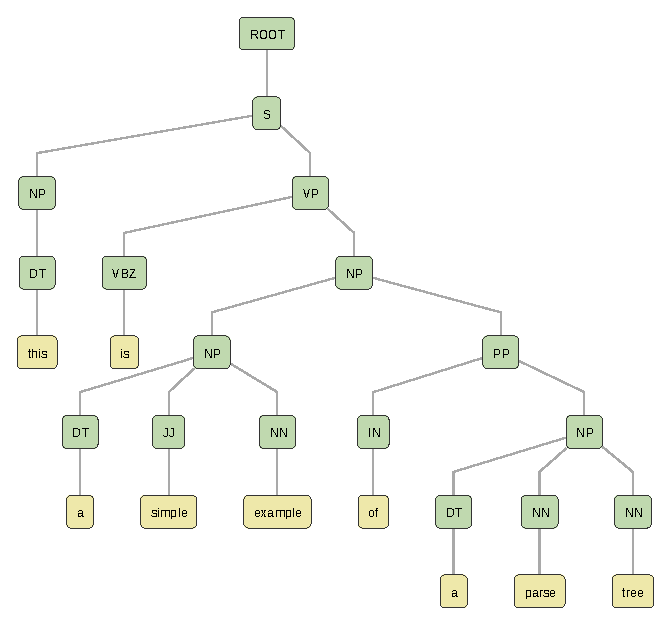
\includegraphics[width=\textwidth]{constparse}}
	\label{fig:consparse}
\end{figure}


\begin{figure}
	\caption{A dependency parse tree for the sentence \natlang{This is a simple example of a parse tree},
		This flattened view may be misleading.
		\natlang{example} is at the peak of the tree, with direct children	being:
		\natlang{this},\natlang{is},\natlang{a},\natlang{simple},
		and \natlang{tree}.
		\natlang{tree} has direct children being: \natlang{of},\natlang{a}, and \natlang{parse}.
	}
	\centering{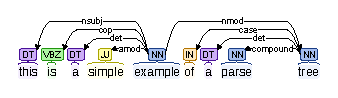
\includegraphics[width=\textwidth]{depparse}}
	\label{fig:depparse}
\end{figure}



Tree structured networks work by applying a recursive unit (which we will call RV) function across pairs (or other groups) of the representations of the lower levels, to produce a combined representation.
The network structure for an input of binary tree structured text is itself a binary tree of RVs.
Each RV (i.e. node in the graph) can be defined by the composition function:
\begin{align}
	\d f_{RV}(\v u, \v v) &= \varphi\left(\left[\begin{array}{cc}
	S & R\end{array}\right]\left[\begin{array}{c}
	\v u\\
	\v v
	\end{array}\right] + \v b \right) \\ \label{equ:rnn1}
			     &= \varphi\left( S\v u +R\v v + \v b \right)
\end{align}
where $\v u$ and $\v v$ are the left and right substructures embeddings (word embeddings at the leaf node level), and $S$ and $R$ are the matrices defining how the left and right children's representations are to be combined.


This is a useful form as all constituency parse trees can be converted into binary parse trees, via left-factoring or right factoring (adding new nodes to the left or right to take some of the children).
This is sometimes called binarization, or putting them into  Chomsky normal form.
This form of structured network has been used in many words, including \tcite{socher2010PhraseEmbedding}, \textcite{SocherEtAl2011:RAE},  \textcite{SocherEtAl2011:PoolRAE},
 \textcite{Socher2011ParsingPhrases} and \textcite{zhang2014BRAE}.
Notice that $S$ and $R$ matrices are shared for all RVs, so all substructures are composed in the same way, based only on whether they are on the left, or the right.

\subsection{Dependency Tree}\label{sec:dependency-tree}
The dependency tree is the other commonly considered parse-tree.
Structured networks based upon the dependency tree have been used by \tcite{socherDTRNN}, \tcite{iyyer2014neural}, and \tcite{iyyer2014generating}.
In these works rather than a using composition matrix for left-child and right-child,
the composition matrix varies depending on the type of relationship of between the head word and its child.
Each dependency relationship type has its own composition matrix.
That is to say there are distinct composition matrices for each of
\natlang{nsub}, \natlang{det}, \natlang{nmod}, \natlang{case} etc.
This allows for multiple inputs to a single head node to be distinguished by their relationship, rather than their order.
This is important for networks using a dependency parse tree structure as the relationship is significant, and the structure allows a node to have any number of inputs.

\aside[Extended example]{
The full example for the $\d f_{RV}(9)$ from \Cref{equ:rvdep} is:
\begin{align*}
 &\d f_{RV}(9) = \varphi(
 	\d W_{head} \i C_{\natlang{tree}} \\
 &+ \d W_{compound}(\d W_{head} \i C_{\natlang{parse}} {+} \v b)\\
 &+ \d W_{det} (\d W_{head} \i C_{\natlang{a}}  + \v b)\\
 &+ \d W_{case}(\d W_{head} \i C_{\natlang{of}}  + \v b)\\
 &+ \v b)
\end{align*}
This in turn would be composed as part of $\d f_{RV}(5)$ for the whole tree headed by 
$\n w_5=\natlang{example}$.
The output of each RV is a representation of that substructure.
}

\aside[No gates\\ No long-term memory]{
	We note that a limitation of most structural models, compared to the sequential RNNs,
	is their lack of explicit gating on memory (e.g. as in GRU and LSTM).
	Any given path down a tree can be looked at as a simple RNN comprised only of basic recurrent units.
	However, these paths are much shorter (being the logarithm of) than the full sequential length of the sentence,
	which offsets the need for such gating.
	Recall that the gating is to provide the longer short term memory.
}



Consider a function $\pi(i,j)$ which returns the relationship between the head word at position $i$ and the child word at position $j$.
For example, using the tree shown in \Cref{fig:depparse}, which has $\n w_8=\natlang{parse}$ and $\n w_9=\natlang{tree}$ then  $\pi(8,9)=\natlang{compound}$.
This is used to define the composed representation for each RV:
\begin{equation}
	\d f_{RV}(i) = \varphi\left(
		\d W_{head} \i C_{\n w_i} 
		+ \sum_{\mathclap{j \in \mathrm{children}(i)}} \d W_{\pi(i,j)} \, f_{RV}(j) + \v b \right)
		\label{equ:rvdep}
\end{equation}
Here $\i C_{\n w_i}$ is the word embedding for $\n w_i$, and $\d W_{head}$ encodes the contribution of the headword to the composed representation.
Similarly, $\d W_{\pi(i,j)}$ encodes the contribution of the child words.
Note that the terminal case is just $f_{RV}(i) = \varphi \left( \d W_{head} \i C_{\n w_i} + \v b \right)$ when a node $i$ has no children.
This use of the relationship to determine the composition matrix,  increases both the networks expressiveness, and also handles the non-binary nature of dependency trees.


A similar technique could be applied to constituency parse trees.
This would be using the part of speech (e.g. VBZ, NN) and phrase tags (e.g. NP, VP) for the sub-structures to choose the weight matrix.
This would, however, lose the word-order information when multiple inputs have the same tag.
This would be the case, for example, in the right-most branch shown in \Cref{fig:consparse}, where both \natlang{parse} and \natlang{tree} have the NN POS tag, and thus using only the tags, rather than the order would leave \natlang{parse tree} indistinguishable from \natlang{tree parse}.
This is not a problem for the dependency parse, as word relationships unambiguously correspond to the role in the phrase's meaning.
As such, allowing the dependency relationship to define the mathematical relationship, as encoded in the composition matrix, only enhances expressibility.



For even greater capacity for the inputs to control the composition,
would be to allow every word be composed in a different way.
This can be done by giving the child nodes there own composition matrices, to go with there embedding vectors.
The composition matrices encode the relationship, and the operation done in the composition.
So not only is the representation of the (sub)phrase determined by a relationship between  its constituents (as represented by their embeddings),
but the nature of that relationship (as represented by the matrix) is also determined by those same constituents.
In this approach at the leaf-nodes, every word not only has a word vector, but also a word matrix.
This is discussed in \Cref{sec:matrix-vector-models}.



\subsection{Parsing} \label{sec:parsing}

The initial work for both contingency tree structured networks  \parencite{socher2010PhraseEmbedding} and for dependency tree structured networks \pcite{stenetorp2013transition} was on the creation of parsers.
This is actually rather different to the works that followed.
In other works the structure is provided as part of the input (and is found during preprocessing).
Whereas a parser must induce the structure of the network,
from the unstructured input text.
This is simpler for contingency parsing, than for dependency parsing.

\aside[The finer detail of parsing]{
Parsing is one of the most well studied problems in computational linguistics.
Presented here is only the highest level overview.
For more details on this,
we recommend consulting the source materials.
Ideally, with reference to a good traditional (that is to say non-neural network based)
NLP textbook, such as: \textcite{manning1999foundations}.
}

\aside[Getting the Embeddings out of the Parser]{
	The implementation of \tcite{socher2010PhraseEmbedding}, is publicly available.
	However, it does not export embeddings.
	It is nested deep inside the Stanford Parser, and thus accessing the embeddings is not at all trivial.}

When creating a binary contingency parse tree, any pair of nodes can only be merged if they are adjacent.
The process described by \textcite{socher2010PhraseEmbedding}, is to consider which nodes are to be composed into a higher level structure each in turn.
For each pair of adjacent nodes, an RV can be applied to get a merged representation.
A linear scoring function is also learned, that takes a merged representation and determines how good it was.
This is trained such that correct merges score highly.
Hinge loss is employed for this purpose.
The Hinge loss  function works on similar principles to negative sampling (see the motivation given in \Cref{sec:negative-sampling}).
Hinge loss is used to cause the merges that occur in the training set to score higher than those that do not.
To perform the parse, nodes are merged;
replacing them with their composed representation;
 and the new adjacent pairing score is then recomputed.
\textcite{socher2010PhraseEmbedding} considered both greedy, and dynamic programming search to determine the order of composition, as well as a number of variants to add additional information to the process.
The dependency tree parser extends beyond this method.


Dependency trees can have child-nodes that do not correspond to adjacent words (non-projective language).
This means that the parser must consider that any (unlinked) node be linked to any other node.
Traditional transition-based dependency parsers function by iteratively predicting links (transitions) to add to the structure based on its current state.
\textcite{stenetorp2013transition}  observed that a composed representation similar to \Cref{equ:rnn1}, was an ideal input to a softmax classifier that would predict the next link to make.
Conversely, the representation that is suitable for predicting the next link to make, is itself a composed representation.
Note, that \textcite{stenetorp2013transition} uses the same matrices for all relationships (unlike the works discussed in \Cref{sec:dependency-tree}).
This is required, as the relationships must be determined from the links made, and thus are not available before the parse.
\tcite{bowman2016fast}, presents a work an an extension of the same principles, which combines the parsing step with the processing of the data to accomplish some task, in their case detecting entailment.



\subsection{Recursive Autoencoders}
\aside[Application to image retrieval]{An interesting application of structured networks was shown in \textcite{socherDTRNN}.
	A dependency tree structured network was trained on a language modelling task (not as a recursive autoencoder, although that would also have been a valid option).
	Then, separately a convolutional neural network was trained to produce a vector output of the same dimensionality -- an image embedding -- such that its distance to its caption's composed vector representation was minimised.
	The effect of this was that images and their captions are projected to a common vector space.
	This allowed for smart image retrieval, from descriptions, by having a set of all images, and storing their embedding representations.
	Then for any query, the sentence embedding can be found and the vector space of images can be searched for the nearest.
	The reverse is not generally as useful, as one can't reasonably store all possible captions describing an image, so as to be able to search for the best one for a user provided image.
	This process of linking a sequence representation to an image embedding is not restricted to structured networks, and can be done with any of the representation methods discussed in this chapter.
	Further, as discussed in \Cref{sec:aligning-vector-spaces-across-languages} it can also be done using pretrained embedding on both sides through (kernel) CCA.
}

\aside[Unfolding RAE implementation]{
	The implementation, and a pretrained model, of the unfolding recursive autoencoder of 
	\textcite{SocherEtAl2011:PoolRAE}
	is available online at \url{https://tinyurl.com/URAE2011}.
	It is easy to use as a command-line Matlab script to generate embeddings.
}

Recursive autoencoders are autoencoders, just as the autoencoder discussed in \Cref{sec:bottle-necking-autoencoder}, they reproduce their input.
It should be noted that unlike the encoder-decoder RNN discussed in \Cref{sec:vae-and-encoder-decoder},
they cannot be trivially used to generate natural language from an arbitrary embeddings, as they require the knowledge of the tree structure to unfold into.
Solving this would be the inverse problem of parsing (discussed in \Cref{sec:parsing}).

The models presented in \textcite{SocherEtAl2011:PoolRAE} and \textcite{iyyer2014generating}
are unfolding recursive autoencoders.
In these models an identical inverse tree is defined above the highest node.
The loss function is the sum of the errors at the leaves, i.e. the distance in vector space between the reconstructed words embeddings and the input word-embeddings.
This was based on a simpler earlier model: the normal (that is to say, not unfolding) recursive autoencoder.


The normal recursive autoencoder,
as used in \textcite{SocherEtAl2011:RAE} and \textcite{zhang2014BRAE} only performs the unfolding for a single node at a time during training.
That means that it assesses how well each merge can individually be reconstructed, not the success of the overall reconstruction.
This per merge reconstruction has a loss function based on the difference between the reconstructed embeddings and the inputs embeddings.
Note that those inputs/reconstructions are not word embeddings: they are the learned merged representations, except when the inputs happen to be leaf node. 
This single unfold loss covers the auto-encoding nature of each merge;
but does not give any direct assurances of the auto-encoding nature of the whole structure.
However, it should be noted that while it is not trained for, the reconstruction components (that during training are applied only at nodes) can nevertheless be applied recursively from the top layer, to allow for full reconstruction.

\subsubsection{Semi-supervised}
In the case of all these autoencoders, except \textcite{iyyer2014generating}, a second source of information is also used to calculate the loss during training.
The networks are being simultaneously trained to perform a task, and to regenerate their input.
This is often considered as semi-supervised learning, as unlabelled data can be used to train the auto-encoding part (unsupervised) gaining a good representation, and the labelled data can be used to train the task output part (supervised)  making that representation useful for the task.
This is done by imposing an additional loss function onto the output of the central/top node.
\begin{itemize}
 \item In \textcite{SocherEtAl2011:RAE} this was for sentiment analysis.
 \item In \textcite{SocherEtAl2011:PoolRAE} this was for paraphrase detection.
 \item In \textcite{zhang2014BRAE} this was the distance between embeddings of equivalent translated phrases of two RAEs for different languages.
\end{itemize}
The reconstruction loss and the supervised loss can be summed, optimised in alternating sequences, or the reconstructed loss can be optimised first, then the labelled data used for fine-tuning.

 


\aside[Sequential models are often preferred to structural models]{
Sequential (RNN) models are much more heavily researched than structural models.
They have better software libraries, are easier to implement, and have more known ``tricks'' (like gates and attention).
In theory it is possible for a sequential model (with sufficiently deep and wide RUs) to internalise the connections that a structural model would possess.
While structural models are theoretically nicer from a linguistics standpoint, pragmatically they are the last resort in modelling.
When attempting to find a useful representation of a sentence for a task, one should first try a sum of word embeddings with a simple network on-top,
then a sequential model (based on LSTM or GRU), and only if these fail then try a structured model.
Arguably before using any neural network approach at all, one should eliminate bag of words, bag of n-grams, the dimensionality reduced version of those bags, and also eliminate LSI and LDA as inputs for the task.
}




\section{Matrix Vector Models}\label{sec:matrix-vector-models}
\subsection{Structured Matrix Vector Model}
\tcite{SocherMVRNN} proposed that each node in the graph should define not only a vector embedding, but a matrix defining how it was to be combined with other nodes.
That is to say, each word and each phrase has both an embedding, and a composition matrix.

Consider this for binary constituency parse trees.
The composition function is as follows:
\begin{align}
\d f_{RV}(\v u, \v v, U, V) &= \varphi\left( [S\; R][U\v v;V\v u] + \v b \right) \\ 
&= \varphi\left( S\,U\v v +R\,V\v u + \v b \right)\\
\d F_{RV}(U, V) &= W\left[U;V\right] = \d W_l U + \d W_r V
\end{align}


$\d f_{RV}$ gives the composed embedding, and $\d F_{RV}$ gives the composing matrix.
The $S$ and $R$ represent the left and right composition matrix components that are the same for all nodes (regardless of content).
The $U$ and $V$ represent the per word/node child composition matrix components.
We note that $S$ and $R$ could, in theory, be rolled in to $U$ and $R$ as part of the learning.
The $\v u$ and $\v v$ represent the per word/node children embeddings,
and $W$ represents the method for merging two composition matrices.

We note that one can define increasingly complex and powerful structured networks along these lines; though one does run the risk of very long training times and of over-fitting.

\subsection{Sequential Matrix Vector Model}
A similar approach, of capturing a per word matrix, 
was used on a sequential model by \tcite{rui2017mvrusemantic}.
While sequential models are a special case of structured models,
it should be noted that unlike the structured models discussed prior,
this matrix vector RNN features a gated memory.
This matrix-vector RNN is an extension of the GRU discussed in \Cref{sec:rnn}, but without a reset gate.


In this sequential model, advancing a time step, is to perform a composition.
This composition is for between the input word and the (previous) state.
Rather than directly between two nodes in the network as in the structural case.
It should be understood that composing with the state is not the same as composing the current input with the previous input.
But rather as composing the current input with all previous inputs (though not equally).

As depicted in \Cref{fig:mvrnn} each word, $\n w_t$ is represented by a word embedding $\nv x_{t}$ and matrix: $\nv X_{\n w_t}$, these are the inputs at each time step.
The network outputs and states are the composed embedding $\n \hat{y}_t$ and matrix $\n Y_t$.

\aside[Remember:]{The product of a matrix with a concatenated vector, is the same as the sum of the two blocks of that matrix each multiplied by the blocks of that vector.}
 

\begin{align}
\n h_t &= \tanh\left(\d W_h [\n x_t; \n \hat{y}_{t-1}] + \dv b_h \right)\\
\n z_t &= \sigma\left(\n Y_{t-1} \n x_t + \n X_t \n \hat{y}_{t-1} + \dv b_z \right)\\
%
\n \hat{y}_t &= \n z_t \odot \n h_t + (1 - \n z_t) \odot \n \hat{y}_{t-1} \\
\n Y_t &= \tanh \left( \d W_Y [\n Y_{t-1}; \n X_t] + \dv b_Y \right)
\end{align}



The matrices $\d W_h$, $\d W_Y$ and the biases $\dv b_h,\; \dv b_z,\; \dv b_Y$ are shared across all time steps/compositions.
$\d W_Y$ controls how the next state-composition $\n Y_t$ matrix is generated from its previous value and the input composition matrix, $\n X_t$;
$\d W_h$ similarly controls the value of the candidate state-embedding $\n h_t$.

$\n h_t$ is the candidate composed embedding (to be output/used as state).
$z_t$ is the update gate, it controls how much of the actual composed embedding ($\n \hat{y}_t$) comes from the candidate $\n h_t$ and how much comes from the previous value ($\n \hat{y}_{t-1}$).
The composition matrix $\n Y_t$ (which is also part of the state/output) is not gated.

Notice, that the state composition matrix $\n Y_{t-1}$ is only used to control the gate $\n z_t$, not to directly affect the candidate composited embedding $\n h_t$.
Indeed, in fact one can note that all similarity to the structural method of \textcite{SocherMVRNN} is applied in the gate $\n z_t$.
The method for calculating $\n h_t$ is similar to that of a normal RU.



\begin{figure}
	\caption{A Matrix Vector recurrent unit}
	\label{fig:mvrnn}
	\begin{adjustbox}{max width=\textwidth}
		\begin{tikzpicture}[]
		\node(hidden)[layer]{$\n h_t = \tanh\left(\d W_h [\n x_t; \n \hat{y}_{t-1}] + \dv b_h \right)$};
		\node(update)[layer, left=of hidden]{$\n z_t = \sigma\left(\n Y_{t-1} \n x_t + \n X_t \n \hat{y}_{t-1} + \dv b_z \right)$};
		\node(state)[layer, above = 6 of update]{$\n \hat{y}_t = \n z_t \odot \n h_t + (1 - \n z_t) \odot \n \hat{y}_{t-1}$};
		
		\node(matrix)[layer, above left = of update]{$\n Y_t = \tanh \left( \d W_Y [\n Y_{t-1}; \n X_t] + \dv b_Y \right)$};
		
		\draw[->] (update) edge node[labe] {$\n z_{t}$} (state.south);		
		\draw[->] (hidden) edge node[labe] {$\n h_{t}$} (state.south);
		
		
		
		\node(in)[below = 6 of update]{input};
		\node(inX)[above = 0 of in.north west]{$\n X_t$};
		\node(inx)[above = 0 of in.north east]{$\n x_t$};
		
		\draw[->] (inX) edge node[labe] {$\n X_t$} (matrix);
		\draw[->] (inx) edge node[labe] {$\n x_t$} (hidden.340);
		\draw[->] (inx) edge node[labe] {$\n x_t$} (update);
		
		\node(stm)[left = 7 of update]{old state};
		\node(stmY)[below = 0 of stm.south east]{$\n Y_{t-1}$};
		\node(stmy)[below = 0 of stm.south west]{$\n \hat{y}_{t-1}$};
		
		
		\draw[->, bend right] (stmy) edge node[labe] {$\n \hat{y}_{t-1}$} (update.south);
		\draw[->, bend right] (stmy) edge node[labe] {$\n \hat{y}_{t-1}$} (hidden.south);
		\draw[->, bend right=40] (stmy) edge node[labe] {$\n \hat{y}_{t-1}$} (state.south);
		
		\draw[->, bend right, thick] (stmY) edge node[labe] {$\n Y_{t-1}$} (update.200);
		\draw[->, bend right, thick] (stmY) edge node[labe] {$\n Y_{t-1}$} (matrix.south);
				
		
		\node(stp)[above = 2 of state.west]{new state\\i.e output};
		\node(stpY)[below = 0 of stp.south west]{$\n Y_{t}$};
		\node(stpy)[below = 0 of stp.south east]{$\n \hat{y}_{t}$};

		\draw[->] (matrix) edge node[labe] {$\n Y_{t}$} (stpY);
		\draw[->] (state) edge node[labe] {$\n \hat{y}_t$} (stpy);

		
		\node(updatelbl)[labe, above= 0 of update]{Update Gate};
		\node(hiddenlbl)[labe, above= 0 of hidden]{Candidate New State Vector};
		\node(matrixlbl)[labe, above= 0 of matrix]{New State Matrix};
		\end{tikzpicture}
	\end{adjustbox}
\end{figure}

The work of \textcite{rui2017mvrusemantic}, was targeting short phrases.
This likely explains the reason for not needing a forget gates.
The extension is obvious, and may be beneficial when applying this method to sentences 


\section{Conclusion, on compositionality}
It is tempting to think of the structured models as compositional,
and the sequential models as non-compositional.
However, this is incorrect.

The compositional nature of the structured models is obvious:
the vector for a phrase is composed from the vectors of the words that the phrase is formed from.

Sequential models are able to learn  the structures.
For example, learning that a word from $n$ time steps ago is to be remembered in the RNN state, to then be optimally combined with the current word, in the determination of the next state.
This indirectly allows the same compositionality as the structured models.
It has been shown that sequential models are indeed in-practice able to learn such relationships between words \pcite{2017arXiv170909360W}.
More generally as almost all aspects of language have some degree of compositionality, and sequential models work very well on most language tasks, this implicitly shows that they have sufficient representational capacity to learn sufficient degrees of compositional processing to accomplish these tasks.


In fact, it has been suggested that even some unordered models such as sum of word embeddings are able to capture some of what would be thought of as compositional information.
\textcite{RitterPosition} devised a small corpus of short sentences describing containing relationships between the locations of objects.
The task and dataset was constructed such that a model must understand some compositionality, to be able to classify which relationships were described.
\textcite{RitterPosition} tested several sentence representations as the input to a na\"ive Bayes classifier being trained to predict the relationship.
They found that when using sums of high-quality word embeddings as the input,
the accuracy not only exceeded the baseline, but even exceeded that from using representation from a structural model.
This suggests that a surprising amount of compositional information is being captured into the embeddings;
which allows simple addition to be used as a composition rule.
Though it being ignorant of word order does mean it certainly couldn't be doing so perfectly,
however the presence of other words my be surprisingly effective hinting at the word order \parencite{White2016a},
thus allow for more apparently compositional knowledge to be encoded than is expected.



To conclude, the compositionality capacity of many models is not as clear cut as it may initially seem.
Further to that the requirement for a particular task to actually handle compositional reasoning is also not always present, or at least not always a significant factor in practical applications.
We have discussed many models in this section, and their complexity varies significantly.
They range from the very simple sum of word embeddings all the way to the the structured matrix models,
which are some of the more complicated neural networks ever proposed.

\end{document}